% --------------------------------------------------------------
% This is all preamble stuff that you don't have to worry about.
% Head down to where it says "Start here"
% --------------------------------------------------------------
 
\documentclass[12pt]{article}
 
\usepackage[nouppercase,headsepline,footsepline,plainfootsepline]{scrpage2}
\automark{section}
\pagestyle{scrheadings}
%\clearscrheadfoot
\ihead{Math 521\;\; Differentiation}
%\ofoot[\pagemark]{\pagemark}% Optional argument controls chapter-starting pages
\ifoot[(Author)]{{\sl \hfill Meenmo K.}}

\usepackage[margin=1in]{geometry} 
\usepackage{amsmath,amsthm,amssymb,scrextend}
\usepackage{fancyhdr}
\usepackage{enumitem}
\usepackage{amsmath}
\usepackage{amssymb}
\usepackage{textcomp}
\usepackage{fancybox}
\usepackage{tikz}
\usepackage{cancel}
\usepackage{tasks}


\newcommand{\N}{\mathbb{N}}
\newcommand{\Z}{\mathbb{Z}}
\newcommand{\I}{\mathbb{I}}
\newcommand{\R}{\mathbb{R}}
\newcommand{\Q}{\mathbb{Q}}
\renewcommand{\qed}{\hfill$\blacksquare$}
\let\newproof\proof
\renewenvironment{proof}{\begin{addmargin}[1em]{0em}\begin{newproof}}{\end{newproof}\end{addmargin}\qed}
% \newcommand{\expl}[1]{\text{\hfill[#1]}$}
\setlength{\parindent}{0pt}
\newenvironment{theorem}[2][Theorem]{\begin{trivlist}
\item[\hskip \labelsep {\bfseries #1}\hskip \labelsep {\bfseries #2.}]}{\end{trivlist}}
\newenvironment{lemma}[2][Lemma]{\begin{trivlist}
\item[\hskip \labelsep {\bfseries #1}\hskip \labelsep {\bfseries #2.}]}{\end{trivlist}}
\newenvironment{problem}[2][Problem]{\begin{trivlist}
\item[\hskip \labelsep {\bfseries #1}\hskip \labelsep {\bfseries #2.}]}{\end{trivlist}}
\newenvironment{exercise}[2][Exercise]{\begin{trivlist}
\item[\hskip \labelsep {\bfseries #1}\hskip \labelsep {\bfseries #2.}]}{\end{trivlist}}
\newenvironment{reflection}[2][Reflection]{\begin{trivlist}
\item[\hskip \labelsep {\bfseries #1}\hskip \labelsep {\bfseries #2.}]}{\end{trivlist}}
\newenvironment{proposition}[2][Proposition]{\begin{trivlist}
\item[\hskip \labelsep {\bfseries #1}\hskip \labelsep {\bfseries #2.}]}{\end{trivlist}}
\newenvironment{corollary}[2][Corollary]{\begin{trivlist}
\item[\hskip \labelsep {\bfseries #1}\hskip \labelsep {\bfseries #2.}]}{\end{trivlist}}
 
 
\begin{document}
\section{Differentiation}
\subsection{Differentiable Functions}
\begin{block}{\bf Def 5.1}
\begin{itemize}
\item Let $f\colon(a,b)\to \mathbb{R},\; a<b\in\overline{\mathbb{R}}$. $f$ is {\sl differentiable at $x\in(a,b)$} if $\lim\limits_{h\to0}\frac{f(x+h)-f(x)}{h}$ exists. 

\item If this limit exists, 
$$f'(x)=\lim\limits_{h\to 0}\frac{f(x+h)-f(x)}{h}$$ is the {\sl derivative of $f$ at $x$}

\item If $f$ is differentiable at all $x\in(a,b),$ we say $f$ is {\sl differentiable}.
\end{itemize}
\end{block}

\vspace{1\baselineskip}
\begin{block}{\bf Theorem 5.2} Let $f\colon (a,b)\to \mathbb{R}$ be differentiable at $x\in(a,b).$ Then $f$ is continuous at $x$.\end{block}

\vspace{1\baselineskip}

\begin{block}{\sl Proof.}
\begin{itemize}
    \item Let $x_n\to x,$ i.e. $\exists\;$ a sequence $h_n\to 0$ such that $x_n=x+h_m$. Then 
    $$f(x_n)-f(x) =\frac{f(x+h_n)-f(x)}{h_n}\cdot h_n \longrightarrow f'(x)\cdot 0 = 0$$
\end{itemize}
\end{block}

\vspace{1\baselineskip}
\begin{block}{\sl Remark 5.3}
\begin{itemize}
    \item $f$ is differentiable $\Rightarrow\;f$ is continuous.
    \item $f$ is continuous $\nRightarrow\;f$ is differentiable
    \item $\exists\;f\colon\mathbb{R}\to\mathbb{R}$ is continuous such that $f $is not differentiable at any $x\in\mathbb{R}$.
\end{itemize}
\end{block}

\vspace{1\baselineskip}
\begin{block}{\bf Theorem 5.4}Let $f,g\colon (a,b)\rightarrow\mathbb{R},$ differentiable at $x\in(a,b).$ Then
\begin{enumerate}[label=(\roman*)]
    \item $(f+g)(x)$ is differentiable at $x,\; (f+g)'(x)=f'(x)+g'(x).$
    \item $(fg)$ is differentiable at $x,\; (fg)'(x)=f'(x)g(x)+g'(x)f(x).$
    \item $\left(\frac{f}{g}\right)$ is differentiable at $x$ if $g(x)\neq 0,$ and $\left(\frac{f}{g}\right)'(x)=\frac{g(x)f'(x)-f(x)g'(x)}{g(x')^2}$
\end{enumerate}
\end{block}

\vspace{1\baselineskip}
\begin{block}{\sl Proof.}
\begin{enumerate}[label=(\roman*)]
    \item Exercise
    \item Consider $$\frac{(fg)(x+h)-(fg)(x)}{h} = \frac{f(x_h)-f(x))g(x_h)+f(x)(g(x+h)-g(x))}{h}$$
    Note $$\frac{f(x+h)-f(x)}{h}\xrightarrow{\text{$h\to\infty$}} f'(x)$$
    $$\frac{g(x+h)-g(x)}{h}\xrightarrow{\text{$h\to 0$}}  g(x)$$
    $$g(x+h) \xrightarrow{\text{$h\to 0$}} g(x)\text{ as $g$ is continuous at $x$.}$$
    So $$\frac{(fg)(x_h)-(fg)(x)}{h}\to f'(x)g(x)+g(x)g'(x).$$
    
    \item $$\frac{\left(\frac{f}{g}\right)(x+h)-\left(\frac{f}{g}\right)(x)}{h} = \frac{f(x+h)g(x)-f(x)g(x+h)}{hg(x+h)g(x)}$$
    $$=\frac{(f(x+h)-f(x))g(x)+f(x)(g(x)-g(x+h))}{h\cdot g(x+h)g(x)}$$
    $$\longrightarrow \frac{f'(x)g(x)-f(x)g'(x)}{g^2(x)}$$
\end{enumerate}
\end{block}

\vspace{1\baselineskip}
\begin{block}{\bf Example}
\begin{enumerate}[label=(\roman*)]
    \item Let $f(x)=c\in \mathbb{R}.$ Then $\frac{f(x+h)-f(x)}{h} = \frac{c-c}{h}=0\rightarrow 0.$ So $f'(x)=0$.
    \item Let $g(x)=x.$ Then $\frac{g(x+h)-g(x)}{h} = \frac{x+h-x}{h} = 1 \rightarrow 1$ (as $h\to 0$). So $g'(x)=1$.
    \item Suppose we know $\frac{d}{dx} x^n = nx^{n-1}.$ 
    \\Check $\frac{d}{dx}(x^{n+1}) = \frac{d}{dx} (x\cdot x^n) = 1\cdot x^n+xnx^{n-1}=(n+1)x^n.$
\end{enumerate}
\end{block}

\vspace{1\baselineskip}
\begin{block}{\bf Example}
Let $g(x)=\begin{cases}
x \sin\left(\frac{1}{x}\right),\;\;x\neq 0\\
0,\qquad\quad\;\;\; x=0
\end{cases}$
$$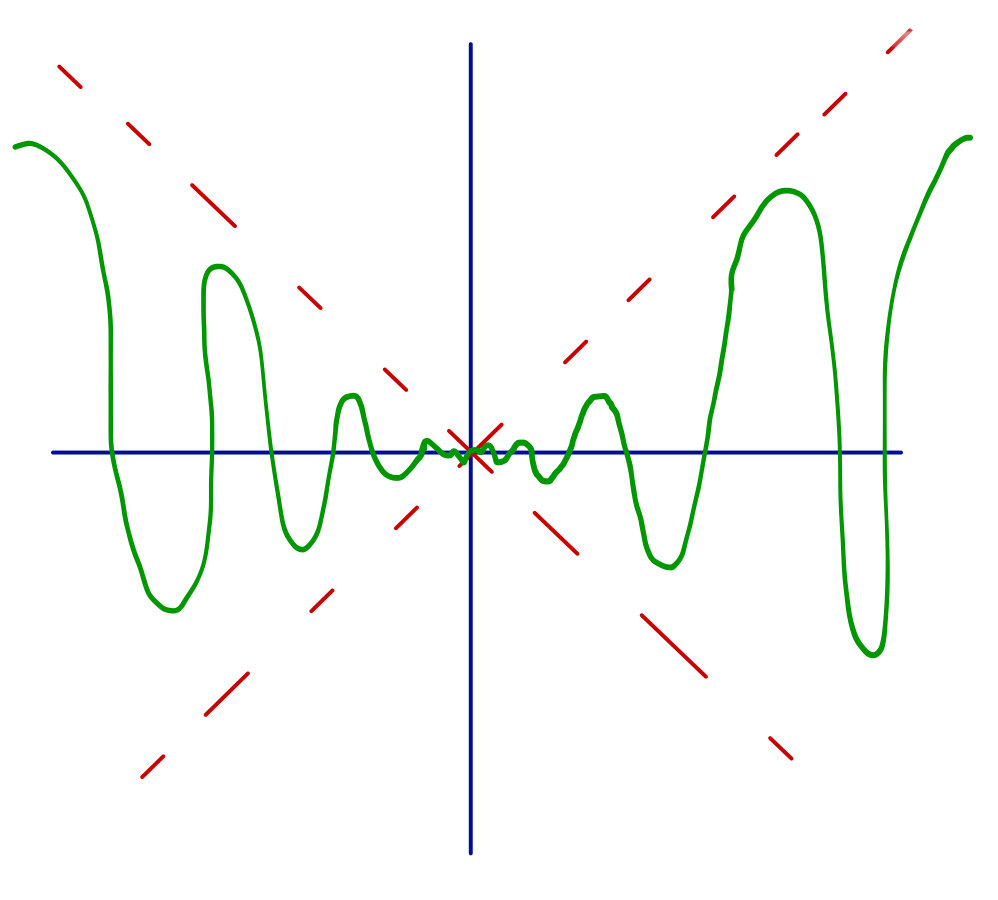
\includegraphics[height=5cm, width=12cm]{Diff_1.jpeg}$$
\begin{itemize}
    \item For $x\neq 0,\; f'(x)=\sin\left(\frac{1}{x}\right)-\frac{1}{x}\cos\left(\frac{1}{x}\right)$.
    \item At $x=0$,
    $$\frac{f(h)-f(0)}{h}=\frac{h\sin\left(\frac{1}{h}\right)}{h}=\sin\left(\frac{1}{h}\right)=$$
    which has no limit as $h\to 0$ (Exercise).
    \item So $f$ is differentiable at all $x\neq 0$.
\end{itemize}
\end{block}

\vspace{1\baselineskip}
\begin{block}{\bf Example}\\ 

\end{block}

\begin{block}{\bf Example}
Let $g(x)=\begin{cases}
x^2 \sin\left(\frac{1}{x}\right),\;\;x\neq 0\\
0,\qquad\quad\;\;\;\;\; x=0
\end{cases}$
\begin{itemize}
    \item Now, if $x\neq 0,\;g'(x)=2x\sin\left(\frac{1}{x}\right)-\cos\left(\frac{1}{x}\right)$.
    \item At $x=0$,
    $$\left|\frac{g(0+h)-g(0)}{h}\right| = \left|\frac{h^2\sin\left(\frac{1}{n}\right)}{h}\right| = \left|h\sin\left(\frac{1}{n}\right)\right| \le |h| \to 0.    $$
    \item So $g'(0)=0$.
\end{itemize}
\end{block}

\vspace{1\baselineskip}
\begin{block}{\bf Theorem}
Let $f\colon(a,b)\rightarrow\mathbb{R},\; f(x)\in(c,d),$ be differentiable at $x\in(a,b)$. Let $g\colon (c,d)\rightarrow\mathbb{R}$ be differentiable at $f(x).$ Then $g\circ f$ is differentiable at $x$ and $(g\circ x)=g'(f(x))f'(x)$ 
\end{block}

\vspace{1\baselineskip}
{\bf Theorem} Chain Rule\\
Let $f:(a,b)\to \mathbb{R},\; f(a,b)\subset(c,d),\; g\colon(c,d)\to \mathbb{R},\; f$ is differentiable at $x\in(a,b)$.\\
$g$ is differentiable at $f(x) \in(C,d),$ then $h=g\circ f\colon(a,b)\to \mathbb{R}$ is differentiable at $x$ and $h'(x)=g'(f(x))\cdot f'(x)$.

\vspace{1\baselineskip}
{\sl Proof.}
\begin{itemize}
  \item Note that as $f$ is differentiable at $x$, $f(x+h)-f(x)=h(f'(x)+u(h)),$ where $u(h)\to 0$ as $h\to 0$.
  \item As $g$ is differentiable at $f(x),\; g(f(x)+k)-g(f(x))=k(g'(f(x))+v(k)),\; v(k)\to 0$ as $k\to 0$.
  \item Consider $g(f(x+h))-g(f(x))=g(f(x)+k)-g(f(x))$ where $k=f(x+h)-f(x)$.\\
    $= k(g'f(x)+v(k)) = (f(x+h)-f(x))(g'(f(x)) +v(f(x+h)-f(x))). = h(f'(x)+u+h))(g'(f(x'))+v(f(x+h)-f(x)))$.
  \item So $\frac{g(f(x+h))-g(f(x))}{h}=(f'(x)+u(h))(g'(f(x))+v(f(x+h)-f(x))) \to f'(x)g'(f(x))$ as $f(x+h)-f(x)\to 0$
  \item Hence $v(f(x+h)-f(x))\to 0$.
\end{itemize}

\section{Mean Value Theorem}
{\bf Definition} Let $f: X\to \mathbb{R}$. We say $x\in X$ is a \underline{local maximum} of $f$ if $\exists\;\delta >0$ such that $\forall\;y\inB_\delta(x),\;f(y)\lef(x).$
We dfine local manimima likewise.\\

{\bf Theorem} Let $f\colon (a,b)\to\mathbb{R}$ have a local maximum at $x\in(a,b)$. Then if $f$ is differentiable at $x,\; f'(x)=0$.\\

{\sl Note.}$x\in (a,b),\; x\neq a,b$\\

{\sl Proof.}
\begin{itemize}
  \item As $x$ is a local maximum, $\exists\;\delta>0$ such that $\forall\;y\in(x-\delta,x+\delta),\; f(y)\le f(x)$.
  \item Let $0<h<\delta.$ Then $\frac{f(x+h)-f(x)}{h}\le 0$ \hfill (1)
  \item $-\delta<h<0$. Then $\frac{f(x+h)-f(x)}{h}\ge 0$. \hfill (2)
  \item From (1), $f'(x)\le 0$. From (2), $f'(x)\ge 0$.
  \mite m Hence $f'(x) = 0$.
\end{itemize}

\vspace{1\baselineskip}
{\bf Theorem} Mean Value Theorem\\
Let $g\colon [a,b]\to\mathbb{R}$ be continuous such that $f$ is differentiable on $(a,b)$. Then $\exists\;x\in(a,b)$ such that $f(b)-f(a) = (b-a)f'(x).$\\ 

{\bf Theorem} Generalized Mean Value Theorem\\
Let $fg\colon [a,b]\to\mathbb{R}$ be continuous and differentiable on $(a,b)$. Then $\exists\; x\in(a,b)$ such that $f(b)-f(a))g'(x)=(g(b)-g(a))f'(x).$\\

\begin{itemize}
    \item Apply MVT to $f$, get $x_1\in (a,b). \; f(b)-f(a)=(b-a)f'(x_1)$ 
    \item With $g,\; \exists x_2\in(a,b),\; g(b)-g(a)=(b-a)g'(x_2)$\\
    \item So $\frac{(f(b)-f(a)}{g(b)-g(a)} = \frac{f'(x_1)}{g'(x_2)}$
\end{itemize}

{\sl Proof.} 

\begin{itemize}
    \item Let $h(t) = (f(b)-f(a))g(t)-(g(b)-g(a))f(t)$
    \item We need to find $x\in(a,b)$ such that $h(x)=0$.
    \item Note $h(a)=(f(b)-f(a))g(a)-(g(b)g(a))f(a) = f(b)g(a)-g(b)f(a)=h(b)$
    \item If $h$ is constant, $h$

    
   \item If not, $\exists\;t\in(a,b)$ such that $h(t)>h(a)$ or $h(t)<h(a)$.
    \item Without loss of generality, $h(t)>h(a)$.
    \item Then as $h$ is continuous on$[a,b]$ by EVT, $\exists\;x\in(a,b),$ such that $h(x)=\max\{h(t)\;|\; t\in[a,b]\}$.
    \item So by the previous theorem, $h'(x)=0$ so done.
\end{itemize}

\vspace{1\baselineskip}
{\bf Theorem} Let $f\colon (a,b)\to\mathbb{R}$ be differentiable.

\begin{enumerate}[label=(\roman*)]
  \item If $f'(x)\ge 0\;\;\forall\;x\in(a,b),\; f$ is monotone increasing.
  \item If $f'(x)\le 0\;\;\forall\;x\in(a,b),\; f$ is monotone decreasing.
  \item If $f'(x)=0\;\;\forall\;x\in(a,b),\; f$ is constant.\\
\end{enumerate}

{\sl Proof.} Homework Exercise.

\vspace{1\baselineskip}
{\bf Theorem} Suppose $f\colon(c,d)\to \mathbb{R}$ differentiable, $c<a<b<d$. If $f'(a) < \lambda < f'(b),\;\exists\;x\in(a,b)$ such that $f'(x)=\lambda$.\\

{\sl Note.} Do not have $f'$ continuous.\\

{\sl Proof.} 
\begin{itemize}
  \item Let $g(t)=f(t)-\lambda t$, so $g'(t)=f'(t)-\lambda.$
  \item Need to find $x\in (a,b)$ such that $g'(x)=0$.
  \item Then $g'(a) = f'(a)-\lambda <0$.
  \item So $\exists\;t\in(a,b)$ such that $g(t_1)<g(a)$.
  \item Also, $g'(b)=f'(b)>\lambda$, so $\exists\; t_2\in(a,b)$ such that $g(t_2)<g(b)$. 
  \item By EVT, $\exists\; x\in[a,b]$ such that $g(x)=\min\{g(t)\;|\;t\in[a,b]\}$
  \item As $g(a)>g(t_1),\;g(t_2)<g(b),\; x\neq a,b$.
  \item So $g(x)=0,\;x\in(a,b)$ as $g'(x)=f'(x)-\lambda$ and we are done.
\end{itemize}
  


\section{L'Hopital's Rule}
{\bf Theorem}\\
Let $f,g\colon(a,b)\to\mathbb{R},$ where $-\infty\lea<b\le \infty,\; f,g$ are differentiable, $g'(x)\neq0\;\;\forall\;x\in(a,b)$ and $\lim\limits_{x\to a} \frac{f'(x)}{g'(x)}=A.$
If either $f(x)\to 0$ and $g(x)\to 0$ as $x\to a$, or $f(x)\to \infty$ and $g(x)\to \infty$ as $x\to a$, then $\lim\limits_{x\to a}\frac{f(x)}{g(x)}=A.$

\newpage
{\bf Example}
\begin{itemize}
  \item $\lim\limits_{x\to 0} \frac{x^2}{x^2} = \lim\limits_{x\to 0} \frac{2x}{2x} = \lim\limits_{x\to 0} \frac{2}{2}=1$
  \item $\lim\limits_{x\to 0} \frac{\sin x}{x} = \lim\limits_{x\to 0} \frac{\cos x}{1} = \frac{\cos 0}{1} = 1$
  \item $\lim\limits_{x\to 0} \frac{\sin x}{\tan x} = \lim\limits_{x\to 0} \frac{\cos x}{\sec^2 x} = \lim\limits_{x\to 0}\cos^3 (x)$
\end{itemize}



\end{document}